%-*-latex-*-
\sectionthree{Sentinel node}
\begin{python0}
from solutions import *; clear()
\end{python0}

A \defone{sentinel node} is a dummy node.
It does not hold data.
Let me show you what I mean.
Look at this singly linked list:

\begin{center}
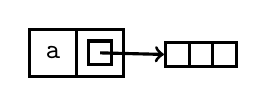
\begin{tikzpicture}

\draw (0.3, 0.3)
  node[draw, line width=0.04cm, , color=black,
       rounded corners=0cm, inner sep=0cm] {

\begin{minipage}[t][0.6cm]{0.6cm}
\mbox{}

\end{minipage}

};\draw (0.3, 0.3) node[color=black] {{\texttt{a}}};
\draw (0.8999999999999999, 0.3)
  node[draw, line width=0.04cm, , color=black,
       rounded corners=0cm, inner sep=0cm] {

\begin{minipage}[t][0.6cm]{0.6cm}
\mbox{}

\end{minipage}

};
\draw (0.9, 0.3)
  node[draw, line width=0.04cm, , color=black,
       rounded corners=0cm, inner sep=0cm] {

\begin{minipage}[t][0.3cm]{0.3cm}
\mbox{}

\end{minipage}

};
\draw (1.88, 0.28)
  node[draw, line width=0.04cm, , color=black,
       rounded corners=0cm, inner sep=0cm] {

\begin{minipage}[t][0.3cm]{0.3cm}
\mbox{}

\end{minipage}

};
\draw (2.1799999999999997, 0.28)
  node[draw, line width=0.04cm, , color=black,
       rounded corners=0cm, inner sep=0cm] {

\begin{minipage}[t][0.3cm]{0.3cm}
\mbox{}

\end{minipage}

};
\draw (2.48, 0.28)
  node[draw, line width=0.04cm, , color=black,
       rounded corners=0cm, inner sep=0cm] {

\begin{minipage}[t][0.3cm]{0.3cm}
\mbox{}

\end{minipage}

};\draw[line width=0.04cm,black,->] (0.9,0.3) to  (1.71,0.28);
\end{tikzpicture}

\end{center}



Suppose I add a dummy node like this:

\begin{center}
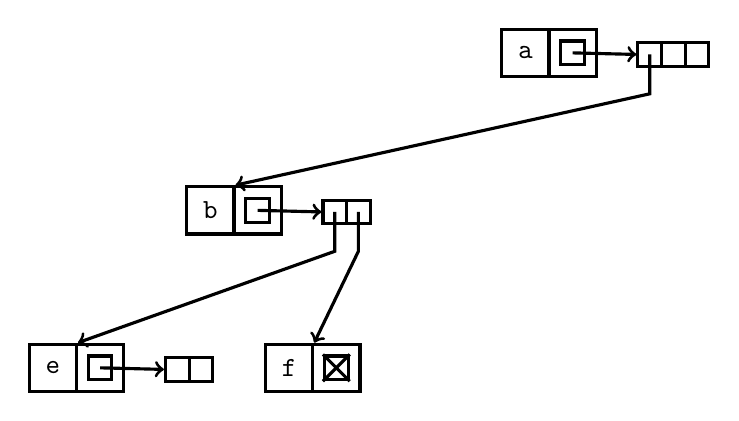
\begin{tikzpicture}

\draw (0.3, 0.3)
  node[draw, line width=0.04cm, , color=black,
       rounded corners=0cm, inner sep=0cm] {

\begin{minipage}[t][0.6cm]{0.6cm}
\mbox{}

\end{minipage}

};\draw (0.3, 0.3) node[color=black] {{\texttt{a}}};
\draw (0.8999999999999999, 0.3)
  node[draw, line width=0.04cm, , color=black,
       rounded corners=0cm, inner sep=0cm] {

\begin{minipage}[t][0.6cm]{0.6cm}
\mbox{}

\end{minipage}

};
\draw (0.9, 0.3)
  node[draw, line width=0.04cm, , color=black,
       rounded corners=0cm, inner sep=0cm] {

\begin{minipage}[t][0.3cm]{0.3cm}
\mbox{}

\end{minipage}

};
\draw (1.88, 0.28)
  node[draw, line width=0.04cm, , color=black,
       rounded corners=0cm, inner sep=0cm] {

\begin{minipage}[t][0.3cm]{0.3cm}
\mbox{}

\end{minipage}

};
\draw (2.1799999999999997, 0.28)
  node[draw, line width=0.04cm, , color=black,
       rounded corners=0cm, inner sep=0cm] {

\begin{minipage}[t][0.3cm]{0.3cm}
\mbox{}

\end{minipage}

};
\draw (2.48, 0.28)
  node[draw, line width=0.04cm, , color=black,
       rounded corners=0cm, inner sep=0cm] {

\begin{minipage}[t][0.3cm]{0.3cm}
\mbox{}

\end{minipage}

};\draw[line width=0.04cm,black,->] (0.9,0.3) to  (1.71,0.28);

\draw (-3.6999999999999997, -1.7)
  node[draw, line width=0.04cm, , color=black,
       rounded corners=0cm, inner sep=0cm] {

\begin{minipage}[t][0.6cm]{0.6cm}
\mbox{}

\end{minipage}

};\draw (-3.6999999999999997, -1.7) node[color=black] {{\texttt{b}}};
\draw (-3.0999999999999996, -1.7)
  node[draw, line width=0.04cm, , color=black,
       rounded corners=0cm, inner sep=0cm] {

\begin{minipage}[t][0.6cm]{0.6cm}
\mbox{}

\end{minipage}

};
\draw (-3.0999999999999996, -1.7)
  node[draw, line width=0.04cm, , color=black,
       rounded corners=0cm, inner sep=0cm] {

\begin{minipage}[t][0.3cm]{0.3cm}
\mbox{}

\end{minipage}

};
\draw (-2.12, -1.7200000000000002)
  node[draw, line width=0.04cm, , color=black,
       rounded corners=0cm, inner sep=0cm] {

\begin{minipage}[t][0.3cm]{0.3cm}
\mbox{}

\end{minipage}

};
\draw (-1.8199999999999998, -1.7200000000000002)
  node[draw, line width=0.04cm, , color=black,
       rounded corners=0cm, inner sep=0cm] {

\begin{minipage}[t][0.3cm]{0.3cm}
\mbox{}

\end{minipage}

};\draw[line width=0.04cm,black,->] (-3.1,-1.7) to  (-2.29,-1.72);

\draw (-5.7, -3.6999999999999997)
  node[draw, line width=0.04cm, , color=black,
       rounded corners=0cm, inner sep=0cm] {

\begin{minipage}[t][0.6cm]{0.6cm}
\mbox{}

\end{minipage}

};\draw (-5.7, -3.6999999999999997) node[color=black] {{\texttt{e}}};
\draw (-5.1, -3.6999999999999997)
  node[draw, line width=0.04cm, , color=black,
       rounded corners=0cm, inner sep=0cm] {

\begin{minipage}[t][0.6cm]{0.6cm}
\mbox{}

\end{minipage}

};
\draw (-5.1, -3.7)
  node[draw, line width=0.04cm, , color=black,
       rounded corners=0cm, inner sep=0cm] {

\begin{minipage}[t][0.3cm]{0.3cm}
\mbox{}

\end{minipage}

};
\draw (-4.119999999999999, -3.72)
  node[draw, line width=0.04cm, , color=black,
       rounded corners=0cm, inner sep=0cm] {

\begin{minipage}[t][0.3cm]{0.3cm}
\mbox{}

\end{minipage}

};
\draw (-3.8199999999999994, -3.72)
  node[draw, line width=0.04cm, , color=black,
       rounded corners=0cm, inner sep=0cm] {

\begin{minipage}[t][0.3cm]{0.3cm}
\mbox{}

\end{minipage}

};\draw[line width=0.04cm,black,->] (-5.1,-3.7) to  (-4.29,-3.72);

\draw (-2.7, -3.6999999999999997)
  node[draw, line width=0.04cm, , color=black,
       rounded corners=0cm, inner sep=0cm] {

\begin{minipage}[t][0.6cm]{0.6cm}
\mbox{}

\end{minipage}

};\draw (-2.7, -3.6999999999999997) node[color=black] {{\texttt{f}}};
\draw (-2.1, -3.6999999999999997)
  node[draw, line width=0.04cm, , color=black,
       rounded corners=0cm, inner sep=0cm] {

\begin{minipage}[t][0.6cm]{0.6cm}
\mbox{}

\end{minipage}

};
\draw (-2.1, -3.7)
  node[draw, line width=0.04cm, , color=black,
       rounded corners=0cm, inner sep=0cm] {

\begin{minipage}[t][0.3cm]{0.3cm}
\mbox{}

\end{minipage}

};\draw[line width=0.04cm,black] (-2.27,-3.53) to  (-1.93,-3.87);
\draw[line width=0.04cm,black] (-1.93,-3.53) to  (-2.27,-3.87);
\draw[line width=0.04cm,black,->] (1.88,0.28) to  (1.88,-0.22) to  (-3.38,-1.38);
\draw[line width=0.04cm,black,->] (-2.12,-1.72) to  (-2.12,-2.22) to  (-5.38,-3.38);
\draw[line width=0.04cm,black,->] (-1.82,-1.72) to  (-1.82,-2.22) to  (-2.38,-3.38);
\end{tikzpicture}

\end{center}



Note that that key value of the sentinel node is not used.
I'm using the next pointer of the sentinel node as the pointer to
the head node (if there's any).

This dummy node is sometimes called the \defone{head sentinel}.
You can think of the head sentinel node as a fake node.
The main purpose of this node is to point to the head node of the linked list
(if the list is non-empty).

Instead of using a head sentinel node in a singly linked list object:
\begin{console}
class SLList
{
public:
    ... 
private:
    SLNode headsentinel_;
};
\end{console}
another implementation is to use a pointer to a head sentinel node
where the head sentinel node is in the heap:
\begin{console}
class SLList
{
public:
    ... 
private:
    SLNode * pheadsentinel_;
};
\end{console}

You can also attach a \defone{tail sentinel} to the end of the
singly linked list.
Here's an example where I have both head and tail sentinel nodes:
\input{stdout49.tex}
The tail sentinel can then be used as an end-of-singly-linked-list node.
So for a computation that involves iterating over a singly-linked list,
the head sentinel node helps you begin the iteration while the
tail sentinel node helps you stop the iteration.

Here's an implementation of a singly linked list class
where both head and tail sentinel nodes are stored
in the heap:
\begin{console}
class SLList
{
public:
    ... 
private:
    SLNode * pheadsentinel_;
    SLNode * ptailsentinel_;
};
\end{console}

Sentinel nodes can simplify your code by providing greater
uniformity for linked list computations.
For instance if \verb!p! is an \verb!SLNode! pointer that
runs through all the nodes in your linked list,
when using sentinel nodes, 
\verb!p! is always pointing to a node
and is not \verb!NULL!.
When you do not use sentinel nodes,
if your linked list is empty, \verb!p! will begin with
\verb!NULL!.
If your linked list is not empty, the last value of \verb!p!
might be \verb!NULL!.
I'll be using sentinel nodes in the next section.

It's also possible to implement a linked list where
there is one sentinel that acts as both the head and tail sentinel:
\begin{center}
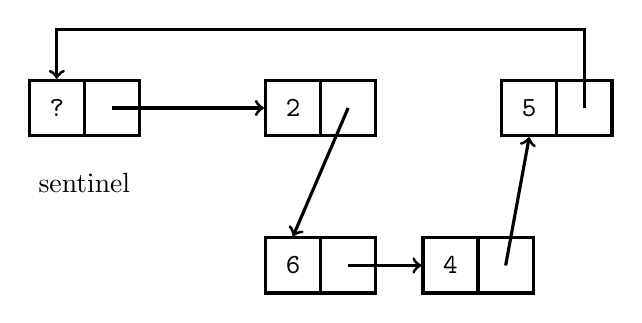
\begin{tikzpicture}

\draw (0.35, 0.35)
  node[draw, line width=0.04cm, , color=black,
       rounded corners=0cm, inner sep=0cm] {

\begin{minipage}[t][0.7cm]{0.7cm}
\mbox{}

\end{minipage}

};\draw (0.35, 0.35) node[color=black] {{\texttt{2}}};
\draw (1.0499999999999998, 0.35)
  node[draw, line width=0.04cm, , color=black,
       rounded corners=0cm, inner sep=0cm] {

\begin{minipage}[t][0.7cm]{0.7cm}
\mbox{}

\end{minipage}

};\draw (1.0499999999999998, 0.35) node[color=black] {{\texttt{}}};
\draw (0.35, -1.65)
  node[draw, line width=0.04cm, , color=black,
       rounded corners=0cm, inner sep=0cm] {

\begin{minipage}[t][0.7cm]{0.7cm}
\mbox{}

\end{minipage}

};\draw (0.35, -1.65) node[color=black] {{\texttt{6}}};
\draw (1.0499999999999998, -1.65)
  node[draw, line width=0.04cm, , color=black,
       rounded corners=0cm, inner sep=0cm] {

\begin{minipage}[t][0.7cm]{0.7cm}
\mbox{}

\end{minipage}

};\draw (1.0499999999999998, -1.65) node[color=black] {{\texttt{}}};
\draw (2.35, -1.65)
  node[draw, line width=0.04cm, , color=black,
       rounded corners=0cm, inner sep=0cm] {

\begin{minipage}[t][0.7cm]{0.7cm}
\mbox{}

\end{minipage}

};\draw (2.35, -1.65) node[color=black] {{\texttt{4}}};
\draw (3.0500000000000003, -1.65)
  node[draw, line width=0.04cm, , color=black,
       rounded corners=0cm, inner sep=0cm] {

\begin{minipage}[t][0.7cm]{0.7cm}
\mbox{}

\end{minipage}

};\draw (3.0500000000000003, -1.65) node[color=black] {{\texttt{}}};
\draw (3.35, 0.35)
  node[draw, line width=0.04cm, , color=black,
       rounded corners=0cm, inner sep=0cm] {

\begin{minipage}[t][0.7cm]{0.7cm}
\mbox{}

\end{minipage}

};\draw (3.35, 0.35) node[color=black] {{\texttt{5}}};
\draw (4.05, 0.35)
  node[draw, line width=0.04cm, , color=black,
       rounded corners=0cm, inner sep=0cm] {

\begin{minipage}[t][0.7cm]{0.7cm}
\mbox{}

\end{minipage}

};\draw (4.05, 0.35) node[color=black] {{\texttt{}}};
\draw (-2.65, 0.35)
  node[draw, line width=0.04cm, , color=black,
       rounded corners=0cm, inner sep=0cm] {

\begin{minipage}[t][0.7cm]{0.7cm}
\mbox{}

\end{minipage}

};\draw (-2.65, 0.35) node[color=black] {{\texttt{?}}};
\draw (-1.9499999999999997, 0.35)
  node[draw, line width=0.04cm, , color=black,
       rounded corners=0cm, inner sep=0cm] {

\begin{minipage}[t][0.7cm]{0.7cm}
\mbox{}

\end{minipage}

};\draw (-1.9499999999999997, 0.35) node[color=black] {{\texttt{}}};\draw[line width=0.04cm,black,->] (-1.95,0.35) to  (-0.02,0.35);
\draw[line width=0.04cm,black,->] (1.05,0.35) to  (0.35,-1.28);
\draw[line width=0.04cm,black,->] (1.05,-1.65) to  (1.98,-1.65);
\draw[line width=0.04cm,black,->] (3.05,-1.65) to  (3.35,-0.02);
\draw[line width=0.04cm,black,->] (4.05,0.35) to  (4.05,1.35) to  (-2.65,1.35) to  (-2.65,0.72);

\draw (-2.3, -0.6)
  node[draw=none, line width=0cm, , color=black,
       rounded corners=0cm, inner sep=0cm] {

\begin{minipage}[t][0.1cm]{0.1cm}
\mbox{}

\end{minipage}

};\draw (-2.3, -0.6) node[color=black] {sentinel};
\end{tikzpicture}

\end{center}


